%Authors guidlines: http://royalsocietypublishing.org/instructions-authors#question5

\documentclass[12pt,letterpaper]{article}

%Packages
\usepackage{pdflscape}
\usepackage{fixltx2e}
\usepackage{textcomp}
\usepackage{fullpage}
%\usepackage{natbib}
\usepackage{float}
\usepackage{latexsym}
\usepackage{url}
\usepackage{epsfig}
\usepackage{graphicx}
\usepackage{amssymb}
\usepackage{amsmath}
\usepackage{bm}
\usepackage{array}
\usepackage[version=3]{mhchem}
\usepackage{ifthen}
\usepackage{caption}
\usepackage{hyperref}
\usepackage{amsthm}
\usepackage{amstext}
\usepackage{enumerate}
\usepackage[osf]{mathpazo}
\usepackage{dcolumn}
\usepackage{lineno}
\usepackage{longtable}
\pagenumbering{arabic}


%Pagination style and stuff
\linespread{2}
\raggedright
\setlength{\parindent}{0.5in}
\setcounter{secnumdepth}{0} 
\renewcommand{\section}[1]{%
\bigskip
\begin{center}
\begin{Large}
\normalfont\scshape #1
\medskip
\end{Large}
\end{center}}
\renewcommand{\subsection}[1]{%
\bigskip
\begin{center}
\begin{large}
\normalfont\itshape #1
\end{large}
\end{center}}
\renewcommand{\subsubsection}[1]{%
\vspace{2ex}
\noindent
\textit{#1.}---}
\renewcommand{\tableofcontents}{}
%\bibpunct{(}{)}{;}{a}{}{,}

%---------------------------------------------
%
%       START
%
%---------------------------------------------

\begin{document}

%Running head
\begin{flushright}
Version dated: \today
\end{flushright}
\bigskip
\noindent RH: Missing morphological data in living mammals

\bigskip
\medskip
\begin{center}

\noindent{\Large \bf Missing morphological data in living mammals}

\bigskip

\noindent {\normalsize \sc Thomas Guillerme$^1$$^,$$^2$$^*$, and Natalie Cooper$^1$$^,$$^2$}\\
\noindent {\small \it 
$^1$School of Natural Sciences, Trinity College Dublin, Dublin 2, Ireland.\\
$^2$Trinity Centre for Biodiversity Research, Trinity College Dublin, Dublin 2, Ireland.}\\
\end{center}
\medskip
\noindent{*\bf Corresponding author.} \textit{Zoology Building, Trinity College Dublin, Dublin 2, Ireland; E-mail: guillert@tcd.ie; Fax: +353 1 6778094; Tel: +353 1 896 2571.}\\
\vspace{1in}

%Line numbering
%\modulolinenumbers[1]
%\linenumbers

%---------------------------------------------
%
%       ABSTRACT
%
%---------------------------------------------

\newpage
\begin{abstract}

\end{abstract}

\noindent ()\\

\vspace{1.5in}

\newpage 

%---------------------------------------------
%
%       INTRODUCTION
%
%---------------------------------------------

\section{Introduction}
%Restrict to two paragraphs?
Studying both living and fossil taxa together in macrovelutionary studies is becoming increasingly common among evolutionary biologists \cite{jacksonwhat2006,quentaldiversity2010,dietlconservation2011,slaterunifying2013,fritzdiversity2013}. One trending method, called Total Evidence allows to combine molecular data from living taxa and morphological data from both living and fossil taxa (e.g. \cite{pyrondivergence2011,ronquista2012,schragocombining2013,slaterunifying2013,beckancient2014,Meseguer01032015}). This promising method allows to apply integrative phylogenetic inference methods such as tip-dating \cite{ronquista2012,Drummond01082012,BEASTmaster}. However, because the Total Evidence method requires a lot of data (both molecular and morphological for both living and fossil taxa), this method has been shown to be sensible to missing morphological data \cite{GuillermeCooper}.

In fact, \cite{GuillermeCooper} demonstrates that when few living taxa coded, topological recovery is bad.
For example, a given phylogeny containing two clades A and B containing only living taxa,
when using a Total Evidence method, molecular data is available for both clades but morphological data is only available for clade A for any reason. Then, the addition of any fossil taxa X related to clade B will lead to a wrong topological placement of this fossil taxa X, branching it somewhere in the clade A instead of the clade B because no morphological data is available to support the placement of the fossil taxa X in clade B.  

%Main rant
If there is no overlapping characters between a living clade and a fossil one, then it is impossible to branch and fossil taxa to that clade. This can be due to evolutionary history (i.e. a fossil angiosperm has no overlapping characters with a living mammal) and is expected. However, this can also be due to missing data (i.e. a fossil primates has no overlapping data with living primates because no data is available for living primates) and will produce artefactual wrong phylogenies (i.e. the fossil primate NOT branching in the primate clade).


\begin{figure}[!htbp]
\centering
    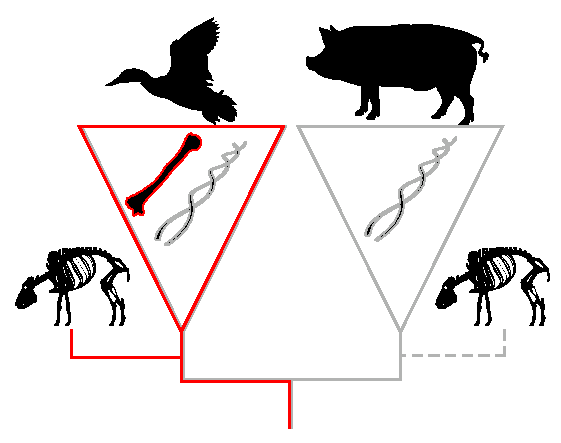
\includegraphics[width=1\textwidth]{MissingDataFigure.pdf}
\caption{Example of topological errors due to missing morphological data in living taxa. If a phylogeny contains two clades, for example Proboscidea and Cetartiodactyla, with molecular data for both but only morphological data for Proboscidea. If an additional Cetartiodactyla fossil (with no molecular data) will be added to the phylogeny, it will erroneously branch with the Proboscidea clade instead of the Cetartiodactyla one.}
\label{Figure_missing_data_problem}
\end{figure}

In this study we investigate the amount of living mammal taxa with available morphological data to assess the potential caveats in building Total Evidence mammal phylogenetic trees. As well as the data availability, we calculate the structure of the data to make sure that clades with a relatively high amount of data are not only containing all taxa from a single clade and none from another clade.

Questions:
\begin{enumerate}
\item{-How many taxa with morphological data are available among each living mammals order?}
\item{-Within each order, how is this data distributed?}
\item{-How can we improve the data coverage in taxa with non random distributed data}
\end{enumerate}


%---------------------------------------------
%
%       METHODS
%
%---------------------------------------------
 
\newpage

\section{Material and Methods}
\subsection{Matrices search}
To investigate the available living taxa with morphological data, we downloaded morphological matrices from three main public databases: morphobank, graeamlloyd.com and rossmounce's github. We downloaded all the matrices containing any fossil or living mammal taxa from these data bases. Additionally we ran a thorough search for matrices that might not have been uploaded on the previously cited data bases through a Google Scholar search. We downloaded the eventual additional morphological matrices from any of the 20 first papers matching with our selected key words and with any of the 35 taxonomic levels (see supplementary materials for detailed description of the procedure). We downloaded 256 % @@@ Number of matrices
matrices containing a total of 9411 % @@@ Number of living OTUs
operational taxonomic units (OTUs) from the combination of both searches (public repositories and Google Scholar).

We then transformed all the matrices to be in the same nexus format. We then standardised the taxonomic nomenclature by fixing invalid binomial inputs to match with the official taxonomic nomenclature rules (i.e. H. sapiens was transformed in Homo sapiens). We assigned each species as being either living or fossil using a taxonomic matching algorithm. We considered living all the OTUs that where either present in Fritz supper tree or in Wilson Reeders taxonomy. We considered fossil all the OTUs that where present in the Paleobiology database. For the OTUs neither labelled as living or fossil we tried to decompose the OTUs name (i.e. $Homo\_sapiens$ became $Homo$ and $sapiens$) and tried to match the to Wilson Reeders taxonomy at any taxonomic level (Family, Genus, $Genus\_species$, etc.). The matching OTUs where labelled as living and the ones still not matching where ignored and labelled as not applicable (NA).

\subsection{Data availability analysis}
\subsubsection{Number of characters threshold}
From all the 256 % @@@ Number of matrices
matrices, we selected only the ones that had at least 100 morphological characters. This arbitrary threshold number of morphological characters was chosen to be in adequacy with \cite{GuillermeCooper} and \cite{harrisonamong-character2014}. Also this threshold avoids biases towards small matrices that could be either not informative (e.g. too few characters) or made of non-applicable characters (e.g. antlers which are sexual dimorphic characters proper to a specific clade).

\subsubsection{Data availability}
To assess the data availability per mammal order, we calculated the percentage of OTUs with morphological data for three different taxonomic level (Family, Genera and Species). We highlighted all the orders containing less than 25\% of living taxa with morphological data because their amount of missing data ($>$75\%) was higher than in \cite{GuillermeCooper} and therefore highly probable of suffering from the effect of missing data. 

\subsubsection{Available data structure}
For the order with no morphological data for all OTUs at the three different taxonomic levels (Family, Genera and Species), we investigated the structure of the available data to test if it was either (i) randomly distributed, (ii) over-dispersed or (iii) clustered. To measure the structure of the available data we used classic community structure metric from the picante R package \cite{picante} where we compared the structure of the available data for each order to the structure of a potentially fully sampled data (i.e. only the OTUs with available morphological data \textit{vs.} all the OTUs).
For each orders and taxonomic level that presented OTUs with no available morphological data, we calculated the Net Relatedness Index (NRI) which quantifies the overall distribution of the data with negative values showing more dispersed data and positive values more clustered data than expected by the null model \cite{webb2002phylogenies}. We choose to present only the NRI values because they have been shown to be slightly less sensitive to the structure of the phylogeny (i.e. branch length and topology) \cite{NRI,journal.pone.0004390} but we also calculated the two other common phylogenetic structure indices: Faith's Phylogenetic Distance (PD)\cite{Faith19921} and the Nearest Taxon Index (NTI) \cite{webb2002phylogenies}. Both metrics are available in the Supplementary results.

%\subsubsection{Data improvement strategy}
%Phylotargeting
%This part as not been done at all! I was looking for a non-GUI version of Arnold and Nunn's software but there is none (Arnold confirmed by email). Therefore because I was focusing on the part above and to make it repeatable I didn't did that part yet. However, I still planing on doing it!

All the following procedure is repeatable and available on GitHub. %Or what is the right way to show it's reproducible?

%---------------------------------------------
%
%       RESULTS
%
%---------------------------------------------

\section{Results}

\subsection{Data availability}
We extracted 1422 living mammal OTUs from the 256 matrices with a minimum of 6 characters and a maximum of 4541. After removing all the matrices with less than 100 the number of extracted living mammals OTUs was down to 815. 11/28 orders have less than 25\% of taxa with morphological data at a species level and 24/28 orders have less than 75\% taxa with available morphological data. At the Genus level however only 3/28 orders have less than 25\% of taxa with morphological data and 16/28 have less than 75\%. Finally, at the family level no order has less than 25\% taxa with available morphological data and only 5/28 have less than 75\% ~\ref{Table_morpho_taxa_proportion}.

\renewcommand\baselinestretch{1.2}\selectfont
\begin{center}
%\caption{Proportion of available OTUs with morphological data per order and per taxonomic level. We highlighted in bold the orders that have more than 75\% of missing data for each taxonomic level. Note that it is possible that more data is available at a higher taxonomic level (Genus $>$ Species) since if the species name for an OTU was not or miss specified, we still counted the OTU for higher taxonomic level analysis.}
% latex table generated in R 3.1.1 by xtable 1.7-3 package
% Mon Feb 23 12:34:36 2015
\begin{longtable}{llll}
  \hline
Order & Taxonomic level & Fraction of OTUs & Percentage of OTUs \\ 
  \hline
Monotremata & Family & 2/2 & 100 \\ 
  Monotremata & Genus & 2/3 & 66.67 \\ 
  Monotremata & Species & 2/4 & 50 \\ 
  Didelphimorphia & Family & 1/1 & 100 \\ 
  Didelphimorphia & Genus & 16/16 & 100 \\ 
  Didelphimorphia & Species & 40/84 & 47.62 \\ 
  Paucituberculata & Family & 1/1 & 100 \\ 
  Paucituberculata & Genus & 2/3 & 66.67 \\ 
  Paucituberculata & Species & 2/5 & 40 \\ 
  Microbiotheria & Family & 1/1 & 100 \\ 
  Microbiotheria & Genus & 1/1 & 100 \\ 
  Microbiotheria & Species & 1/1 & 100 \\ 
  Notoryctemorphia & Family & 1/1 & 100 \\ 
  Notoryctemorphia & Genus & 1/1 & 100 \\ 
  \textbf{Notoryctemorphia} & \textbf{Species} & \textbf{0/2} & \textbf{0} \\ 
  Dasyuromorphia & Family & 2/2 & 100 \\ 
  Dasyuromorphia & Genus & 7/22 & 31.82 \\ 
  \textbf{Dasyuromorphia} & \textbf{Species} & \textbf{8/64} & \textbf{12.5} \\ 
  Peramelemorphia & Family & 2/2 & 100 \\ 
  Peramelemorphia & Genus & 7/7 & 100 \\ 
  Peramelemorphia & Species & 16/18 & 88.89 \\ 
  Diprotodontia & Family & 9/11 & 81.82 \\ 
  Diprotodontia & Genus & 20/38 & 52.63 \\ 
  \textbf{Diprotodontia} & \textbf{Species} & \textbf{16/126} & \textbf{12.7} \\ 
  Afrosoricida & Family & 2/2 & 100 \\ 
  Afrosoricida & Genus & 17/17 & 100 \\ 
  Afrosoricida & Species & 23/42 & 54.76 \\ 
  Macroscelidea & Family & 1/1 & 100 \\ 
  Macroscelidea & Genus & 4/4 & 100 \\ 
  Macroscelidea & Species & 5/15 & 33.33 \\ 
  Tubulidentata & Family & 1/1 & 100 \\ 
  Tubulidentata & Genus & 1/1 & 100 \\ 
  Tubulidentata & Species & 1/1 & 100 \\ 
  Hyracoidea & Family & 1/1 & 100 \\ 
  Hyracoidea & Genus & 1/3 & 33.33 \\ 
  Hyracoidea & Species & 1/4 & 25 \\ 
  Proboscidea & Family & 1/1 & 100 \\ 
  Proboscidea & Genus & 1/2 & 50 \\ 
  Proboscidea & Species & 1/3 & 33.33 \\ 
  Sirenia & Family & 2/2 & 100 \\ 
  Sirenia & Genus & 2/2 & 100 \\ 
  Sirenia & Species & 2/4 & 50 \\ 
  Cingulata & Family & 1/1 & 100 \\ 
  Cingulata & Genus & 8/9 & 88.89 \\ 
  \textbf{Cingulata} & \textbf{Species} & \textbf{6/25} & \textbf{24} \\ 
  Pilosa & Family & 3/5 & 60 \\ 
  Pilosa & Genus & 3/5 & 60 \\ 
  \textbf{Pilosa} & \textbf{Species} & \textbf{3/29} & \textbf{10.35} \\ 
  Scandentia & Family & 2/2 & 100 \\ 
  Scandentia & Genus & 2/5 & 40 \\ 
  \textbf{Scandentia} & \textbf{Species} & \textbf{2/20} & \textbf{10} \\ 
  Dermoptera & Family & 1/1 & 100 \\ 
  Dermoptera & Genus & 1/2 & 50 \\ 
  Dermoptera & Species & 1/2 & 50 \\ 
  Primates & Family & 15/15 & 100 \\ 
  Primates & Genus & 48/68 & 70.59 \\ 
  \textbf{Primates} & \textbf{Species} & \textbf{56/351} & \textbf{15.95} \\ 
  Rodentia & Family & 10/32 & 31.25 \\ 
  \textbf{Rodentia} & \textbf{Genus} & \textbf{20/451} & \textbf{4.43} \\ 
  \textbf{Rodentia} & \textbf{Species} & \textbf{10/2095} & \textbf{0.48} \\ 
  Lagomorpha & Family & 1/2 & 50 \\ 
  \textbf{Lagomorpha} & \textbf{Genus} & \textbf{1/12} & \textbf{8.33} \\ 
  \textbf{Lagomorpha} & \textbf{Species} & \textbf{1/86} & \textbf{1.16} \\ 
  Erinaceomorpha & Family & 1/1 & 100 \\ 
  Erinaceomorpha & Genus & 10/10 & 100 \\ 
  Erinaceomorpha & Species & 21/22 & 95.45 \\ 
  Soricomorpha & Family & 3/4 & 75 \\ 
  Soricomorpha & Genus & 19/43 & 44.19 \\ 
  \textbf{Soricomorpha} & \textbf{Species} & \textbf{19/392} & \textbf{4.85} \\ 
  Chiroptera & Family & 13/18 & 72.22 \\ 
  Chiroptera & Genus & 68/202 & 33.66 \\ 
  \textbf{Chiroptera} & \textbf{Species} & \textbf{108/1054} & \textbf{10.25} \\ 
  Pholidota & Family & 1/1 & 100 \\ 
  Pholidota & Genus & 1/1 & 100 \\ 
  Pholidota & Species & 3/8 & 37.5 \\ 
  Carnivora & Family & 11/15 & 73.33 \\ 
  \textbf{Carnivora} & \textbf{Genus} & \textbf{30/125} & \textbf{24} \\ 
  \textbf{Carnivora} & \textbf{Species} & \textbf{42/283} & \textbf{14.84} \\ 
  Perissodactyla & Family & 3/3 & 100 \\ 
  Perissodactyla & Genus & 6/6 & 100 \\ 
  Perissodactyla & Species & 7/16 & 43.75 \\ 
  Cetartiodactyla & Family & 20/21 & 95.24 \\ 
  Cetartiodactyla & Genus & 76/128 & 59.38 \\ 
  Cetartiodactyla & Species & 106/311 & 34.08 \\ 
   \hline
\hline
\end{longtable}

\label{Table_morpho_taxa_proportion}
\end{center}
\renewcommand\baselinestretch{2}\selectfont

\subsection{Available data structure}
Among the orders containing OTUs with no morphological data, only two orders (Carnivora and Chiroptera) are significantly clustered both at the species and the genus level but not at the family level ~\ref{Table_data_structure}.
\renewcommand\baselinestretch{1.2}\selectfont
\begin{center}
%\caption{Data structure for the orders with OTUs without morphological data per taxonomic level. The the Net Relatedness Index (NRI) is negative, the OTUs are more dispersed than expected by chance (random); when the NRI is positive, the OTUs are more clustered by expected by chance. The p-value indicates the significance in difference from the null model (random).}
% latex table generated in R 3.1.1 by xtable 1.7-3 package
% Fri Feb 27 10:08:44 2015
\begin{longtable}{lllll}
\caption{Data structure for the orders with OTUs without morphological data per taxonomic level. When the Net Relatedness Index (NRI) is negative, the OTUs are more dispersed than expected by chance (random); when the NRI is positive, the OTUs are more clustered by expected by chance. The p-value indicates the significance in difference from the null model (random).} \\ 
  \hline
Order & Taxonomic level & Percentage of OTUs & NRI & p-value \\ 
  \hline
Monotremata & Genus & 66.667 & -0.695 & 0.663 \\ 
  Monotremata & Species & 50 & -0.966 & 0.566 \\ 
  Didelphimorphia & Species & 47.619 & -1.33 & 0.915 \\ 
  Paucituberculata & Genus & 66.667 & -0.756 & 0.682 \\ 
  Paucituberculata & Species & 40 & -0.64 & 0.493 \\ 
  Dasyuromorphia & Genus & 31.818 & -1.102 & 0.894 \\ 
  Dasyuromorphia & Species & 12.5 & -1.098 & 0.93 \\ 
  Peramelemorphia & Species & 88.889 & -0.55 & 0.748 \\ 
  Diprotodontia & Family & 81.818 & -0.349 & 0.551 \\ 
  Diprotodontia & Genus & 52.632 & -0.31 & 0.595 \\ 
  Diprotodontia & Species & 12.698 & -0.975 & 0.849 \\ 
  Afrosoricida & Species & 54.762 & 1.555 & 0.077 \\ 
  Macroscelidea & Species & 33.333 & -0.474 & 0.66 \\ 
  Sirenia & Species & 50 & -0.957 & 0.845 \\ 
  Cingulata & Genus & 88.889 & 1.31 & 0.229 \\ 
  Cingulata & Species & 24 & 0.648 & 0.223 \\ 
  Pilosa & Family & 60 & -0.603 & 0.891 \\ 
  Pilosa & Genus & 60 & -0.877 & 0.795 \\ 
  Pilosa & Species & 10.345 & -1.508 & 0.997 \\ 
  Scandentia & Genus & 40 & -0.747 & 0.639 \\ 
  Scandentia & Species & 10 & -1.259 & 0.984 \\ 
  Primates & Genus & 70.588 & -0.302 & 0.607 \\ 
  Primates & Species & 15.954 & -1.504 & 0.951 \\ 
  Rodentia & Family & 31.25 & 0.113 & 0.395 \\ 
  Rodentia & Genus & 4.435 & -1.032 & 0.848 \\ 
  Rodentia & Species & 0.477 & -0.967 & 0.856 \\ 
  Erinaceomorpha & Species & 95.455 & -0.777 & 0.914 \\ 
  Soricomorpha & Family & 75 & -0.95 & 0.619 \\ 
  Soricomorpha & Genus & 44.186 & 1.157 & 0.116 \\ 
  Soricomorpha & Species & 4.847 & -1.869 & 0.977 \\ 
  Chiroptera & Family & 72.222 & 0.866 & 0.201 \\ 
  \textbf{Chiroptera} & \textbf{Genus} & \textbf{33.663} & \textbf{18.87} & \textbf{0.001} \\ 
  \textbf{Chiroptera} & \textbf{Species} & \textbf{10.247} & \textbf{20.112} & \textbf{0.001} \\ 
  Pholidota & Species & 37.5 & 1.14 & 0.175 \\ 
  Carnivora & Family & 73.333 & 0.517 & 0.285 \\ 
  \textbf{Carnivora} & \textbf{Genus} & \textbf{24} & \textbf{4.014} & \textbf{0.002} \\ 
  \textbf{Carnivora} & \textbf{Species} & \textbf{14.841} & \textbf{17.954} & \textbf{0.001} \\ 
  Perissodactyla & Species & 43.75 & 0.733 & 0.199 \\ 
  Cetartiodactyla & Family & 95.238 & 0.352 & 0.193 \\ 
  Cetartiodactyla & Genus & 59.375 & -3.221 & 1 \\ 
  Cetartiodactyla & Species & 34.084 & -2.768 & 1 \\ 
   \hline
\hline
\label{Table_data_structure}
\end{longtable}

\label{Table_data_structure}
\end{center}
\renewcommand\baselinestretch{2}\selectfont
Two contrasted results are shown on figure~\ref{Figure_example_coverage} with randomly distributed data in Cetartiodactyla (Fig.~\ref{Figure_example_coverage}A) and clustered available data in Carnivora (mainly Canida;e Fig.~\ref{Figure_example_coverage}B). 
\begin{figure}[!htbp]
\centering
    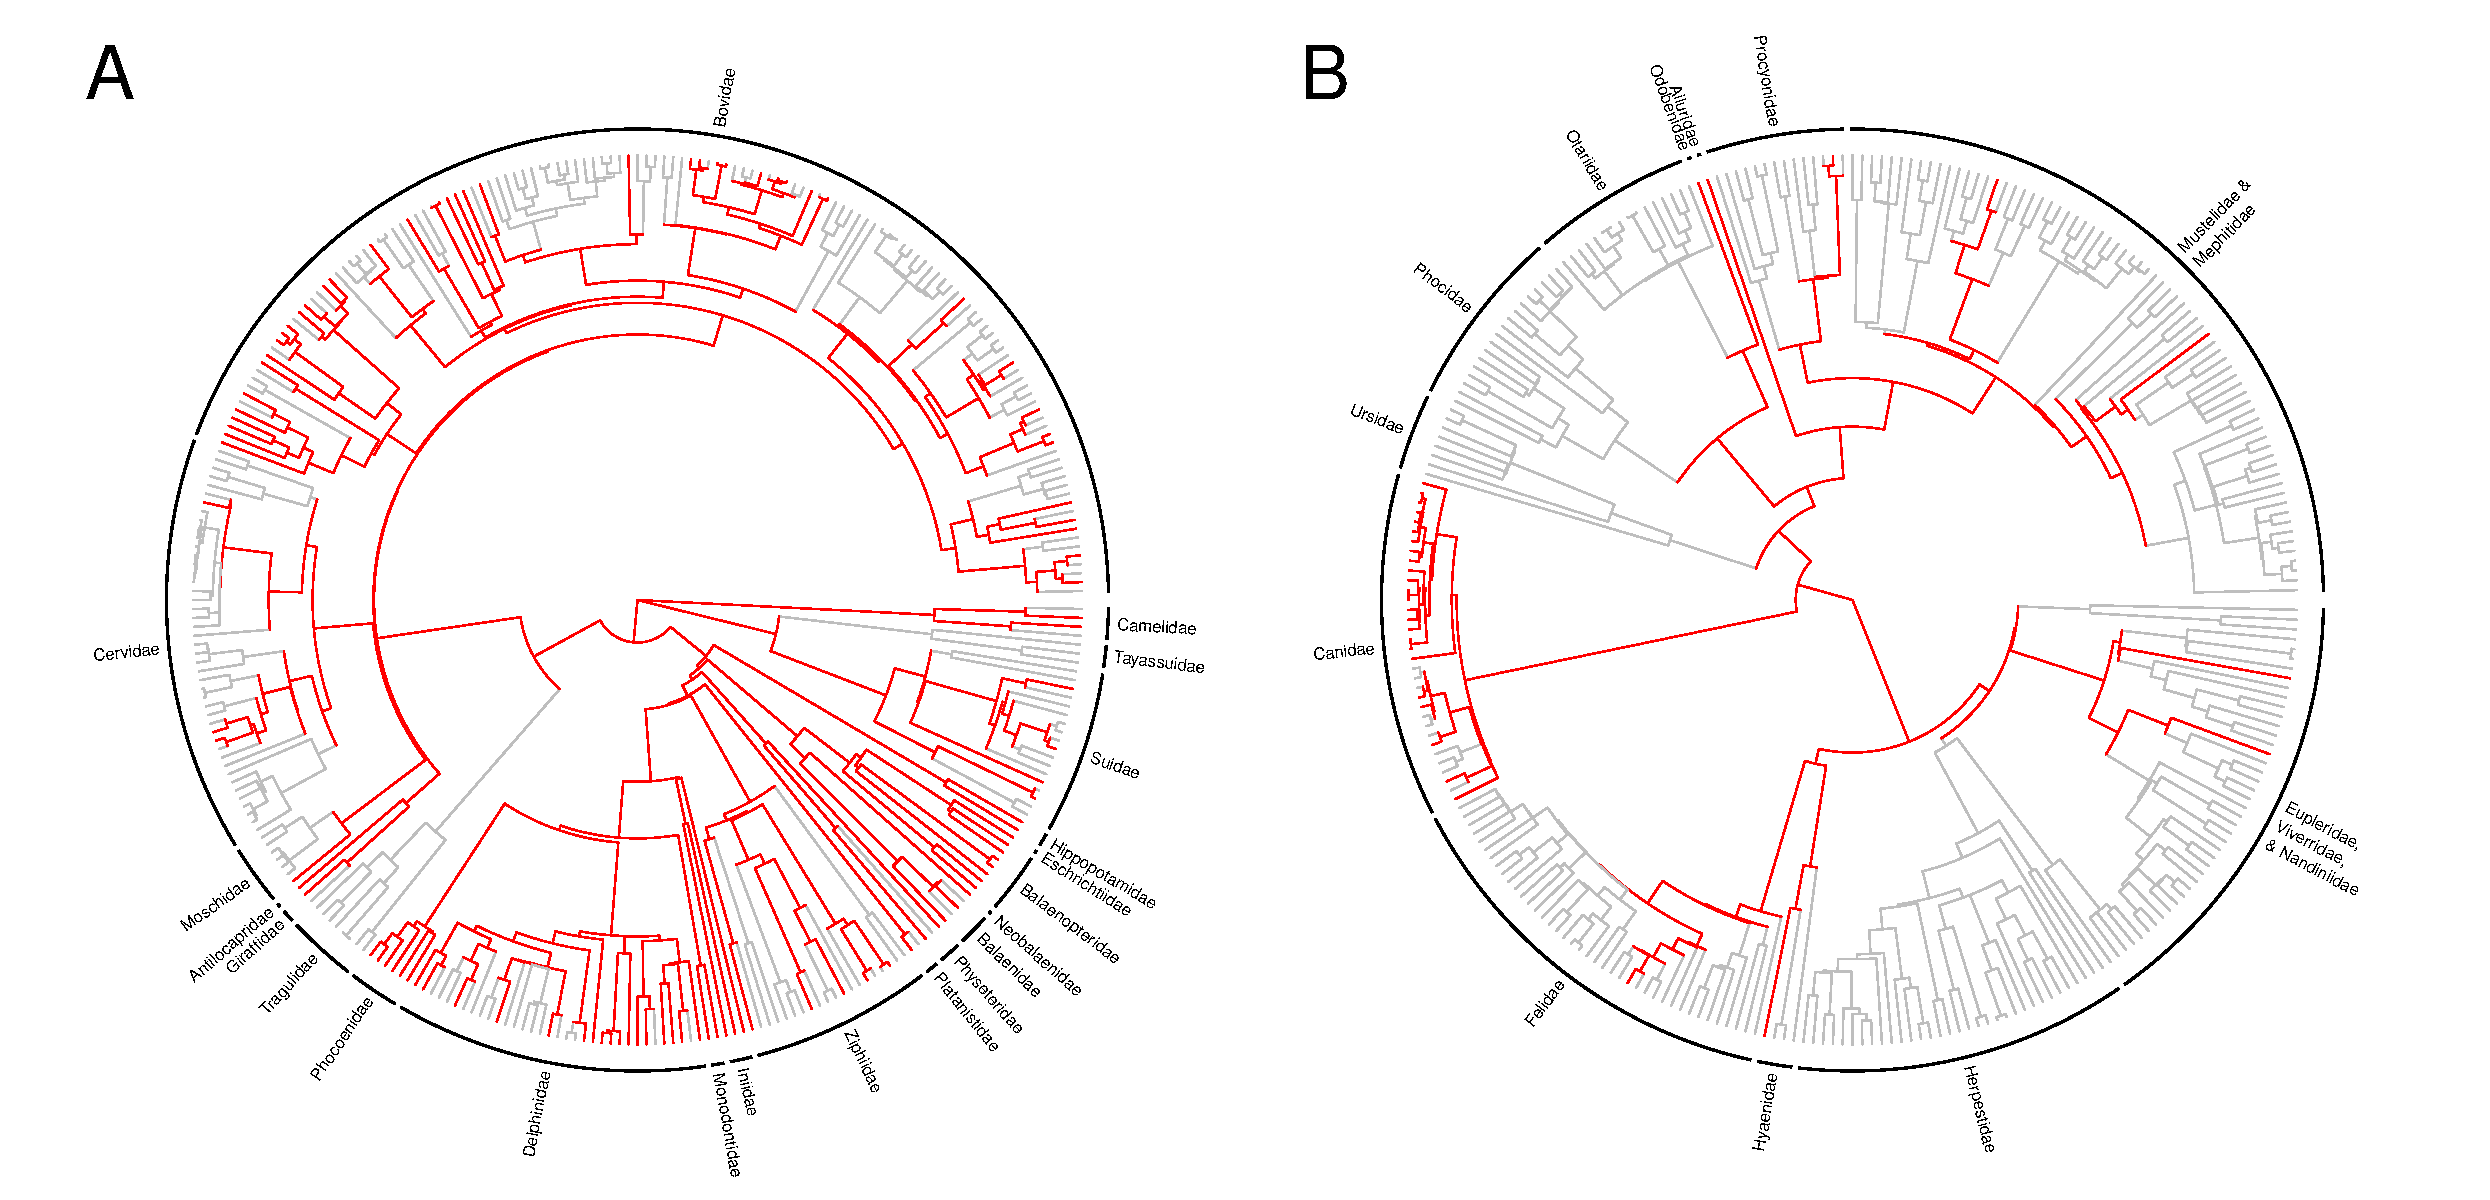
\includegraphics[width=1\textwidth]{example_coverage.pdf}
\caption{Distribution of available morphological data across cetartiodactyles (\textbf{A}) and carnivores (\textbf{B}). Edges are colored in grey when no morphological data is available or in red when data is available.}
\label{Figure_example_coverage}
\end{figure}

%\subsection{Data improvement strategy}


%---------------------------------------------
%
%       DISCUSSION
%
%---------------------------------------------

\section{Discussion}

%\subsection{Data availability}
It's pretty bad

%\subsection{Available data structure}
But good news! It's at least mainly random

%Caveats
However, we counted only the raw number of characters here and not there similarity. It might be that actually the amount of available data here is lower due to non overlap of characters....

%Let's code some data
So let's go coding some data and using opensource traceable data bases like morphobank!



%Biology letters various stuff
\section{Ethics statement}
\section{Data accessibility statement}
All data is available and reproducible on GitHub.
\section{Authors’ contributions statement}
Conceived and designed the experiments: TG NC. Performed the experiments: TG. Analyzed the data: TG. Wrote the paper: TG NC.
\section{Acknowledgements}
Nick Matzke, April Wright, David Bapst and Graeme Lloyd.
\section{Funding statement}
This work was funded by a European Commission CORDIS Seventh Framework Programme (FP7) Marie Curie CIG grant (proposal number: 321696).

\bibliographystyle{vancouver}
\bibliography{References}


\section{SOM}
1- Data collection: key words, clade (ordinal) metacharacters, Google Search terms, Google Search protocol, Google Search rarefaction curve.

\section{search terms}

\subsection{Mammalian orders terms}
The searched mammalian order terms are available in $search_terms_latin.txt$ or $search_terms_meta.txt$. The file containing the meta names is the Latin name files but with replacing the latin suffixes ([ia|ata|ea|a]) by a joker character (*) and by replacing the first letter by a upper/lower case meta character (e.g. [Aa]).

\subsubsection{Ross Mounce data set}
I selected all the matrices containing at least one of the mammalian orders names from Ross Mounce GitHub $cladistic-data/nexus_files$ repository (accessed on the 02/12/2014).

\subsection{Graeme Lloyd}
Selecting the downloadable matrices

\subsection{Morphobank}
\textit{order}

\subsection{Google scholars}
20 first results since 2010 with the following key words:
\textit{order} ("morphology" OR "morphological" OR "cladistic") AND characters matrix paleontology phylogeny
Why 20 first results? Because rarefaction curve, check supplemetaries

\section{Wrong Bionmial names and typos}
I fixed the wrong bionomial names format (e.g. H. sapiens) into the correct ones (e.g. Homo sapiens) manually using the abreviation list in the concerned publications.


\section{Supplementary results}
%Tables
%Figures


%END
\end{document}